\documentclass[letterpaper]{article}
%packages from icwm format
\usepackage{AuthorKit/aaai}
\usepackage{times}
\usepackage{helvet}
\usepackage{courier}

%packages I used
\usepackage{verbatim}
\usepackage{latexsym}
\usepackage{amsmath, amsfonts, amssymb}
\usepackage{graphicx}
\usepackage{url}

\frenchspacing
\setlength{\pdfpagewidth}{8.5in}
\setlength{\pdfpageheight}{11in}
\pdfinfo{
/Title (Automated Vocabulary Creation For Elections)
/Author (Aravindan Mahendiran, Naren Ramakrishnan, Bert Huang, Lise Getoor)}
\setcounter{secnumdepth}{0}  

% stuff copied from Bert's paper
\newcommand{\then}{\Rightarrow}
\newcommand{\softor}{\operatornamewithlimits{\tilde{\vee}}}
\newcommand{\softand}{\operatornamewithlimits{\tilde{\wedge}}}
\newcommand{\softthen}{\operatornamewithlimits{\tilde{\then}}}
\newcommand{\softneg}{\operatornamewithlimits{\tilde{\neg}}}

\def\RVs{\mathbf{X}}
\def\RV{{X}}
\def\rvpt{{\mathbf{x}}}
\def\reals{{\mathbb{R}}}
\def\extReals{{\mathbb{R}^{\infty}}}
\def\potentials{{\phi}}
\def\potential{{\phi}}
\def\prob{{\mathbb{P}}}
\def\density{{f}}
\def\psl{{PSL}}
\def\Cineq{{B}}
\def\Ceq{{A}}
\def\bineq{{b}}
\def\beq{{a}}
\def\domain{{\mathbf{D}}}
\def\kineq{{k_B}}
\def\keq{{k_A}}

\begin{document}
\title{Automated Vocabulary Creation For Elections}
\author{{\bf Aravindan Mahendiran}$^{1}$, {\bf Naren Ramakrishnan}$^{1}$, 
             {\bf Bert Huang}$^{2}$, {\bf Lise Getoor}$^{2}$\\
              $^1$Virginia Tech.,$^2$University of Maryland}
\maketitle
\begin{abstract}
\begin{quote}
Twitter mining over the last few years has garnered a lot of attention from the research community. 
Strong correlations have been shown between Twitter \emph{‘mentions’} and stock markets, book sales and flu outbreaks which is then used for forecasting.
Even though such methodologies are accurate in forecasting the trends to a great extent, their performance is dictated by the domain specific vocabulary is used to track the relevant tweets. 
Such a vocabulary is usually provided by subject matter experts but is not exhaustive.
The language used in Twitter is drastically different from other forms of writing like those in news articles or even web blogs.  
It constantly evolves with time as users adopt popular hashtags to express their opinion.
Thus, the vocabulary used by the forecasting algorithms needs to be dynamic in nature and should capture the rising trends of the domain. 
Otherwise, the prediction algorithms miss out on capturing the some of the most informative documents.
\newline 
We propose a novel unsupervised learning algorithm builds a vocabulary through modeling user preferences by exploiting the explicit and latent structure in such data sets.
We use Probabilistic Soft Logic, a framework for probabilistic reasoning over relational domains, to develop a query expansion algorithm that learns such a dynamic vocabulary for any given domain.  
Using 7 presidential elections from Latin America we show how such a query expansion methodology improves the recall and accuracy of two state of the art election prediction algorithms. 
Through this approach we achieve close to 2x increase in the recall and 15.5\% reduction in the prediction error. 
\end{quote}
\end{abstract}
\section{INTRODUCTION}
The last decade has seen a massive explosion of on-line data in all forms be it news articles, blogs or social media like Twitter, Facebook and MySpace.
Twitter is a novel micro-blogging service and was launched in 2006.
Twitter users post messages called tweets on a public message board  and these tweets are limited to 140 characters.
Originally the tweets were meant to be personal status updates but over the years these tweets have evolved into much more.
Now apart from simple status updates, tweets can be URLs websites or even directed messages to particular individuals.
Due to the short nature of the messages users often combine multiple words into \emph{hashtags} to convey their views.
Therefore, these hashtags become the most important part of a tweet as the entire essence of the tweet is captured in single hashtag.. 
These hashtags evolve over time and gain more traction as users adopt the popular ones.
This makes the language used in Twitter very different from other textual web content like blogs and articles.
\newline
Today twitter has grown so big\footnote{As of May 7,2013 twitter has 555 million active registered users with 135000 new users signing up everyday and approximately 1 billion tweets created every 5 days}
that it has come to be looked at as a treasure trove of mine-able data.
With official APIs that are open to public, the easy access to large volumes of data has piqued the interest of scientists in the data mining community.
Researchers have studied various real world phenomenon like book sales, box office earnings and even stock prices and have not only shown that they have  strongs correlations to the chatter on Twitter ~\cite{gruhl2005predictive,asur2010predicting,bollen2011twitter}
but were also able to make forecasts about future trends too.
\paragraph{}
However, the more curious research is whether the on-line chatter be used to model the social, economic and political landscape of a country.
Political leaders have started using Twitter as a channel to mobilize supporters for their ideologies.
For the 2008 US presidential election Barack Obama used social media and specifically Twitter extensively in his campaign. 
His victory established Twitter as a channel to garner support for a particular idealogy be it political or otherwise.
Bollen et al. ~\cite{bollen2011modeling} used a version of the well-established psychometric instrument- Profile of Mood States(POMS) to model the mood of twitter traffic and correlate it to a number of social and economic events that occurred during the same time period. 
The results from this research instigated more researchers to study and quantify the political sentiment through social media and if possible even forecast election results.
However, there is a constant debate among political scientists on whether Twitter can be used as a surrogate for political opinion of the masses.
Some believe twitter indeed is an indicator of political opinions, while others question the validity of such results.. 
In this work we aim to answer these questions by trying to improve the performance of election prediction algorithms that use Twitter.
The following section reviews the current state of the art approaches to election prediction. 

\section{RELATED WORK}
We divide the literature review into four parts.
First we look at a selection of volume based approaches to predict elections i.e., models that predict election results by merely counting the number of times a particular candidate is mentioned in Twitter.
Then we review more sophisticated approaches that model the demographics of an election to make more informed predictions.
In the third section, we shall summarize a quite prevalent pessimistic view on such methodologies' capability to predict elections.
Lastly we review Probabilistic Soft Logic, a framework we use to build a vocabulary dynamically.
\subsection{Volume based approaches}
In one of the most cited papers in this space, ~\cite{tumasjan2010predicting} the authors claim that 
\emph{ "The mere number of tweets reflect voter preferences and comes close to  traditional polls.."}
while predicting  the 2010 German federal election. % by counting candidate mentions on twitter.
They go on to strongly conclude that Twitter can indeed be a valid indicator of political opinion.
This was followed by ~\cite{o2010tweets,saez2011total,bermingham2011using,demartini2011analyzing} all of which use volume based approaches combined with sentiment analysis.
Both ~\cite{o2010tweets,bermingham2011using} fit a regression model to opinion polls with volume of mentions and sentiment as independent variables and the opinion polls as the dependant variable. 
They conclude that sentiment is a weak predictor compared to share of volume.
\newline In general the methodologies described in these publications count the occurrence of certain hand filtered keywords in the "Twittersphere" and classify such tweets as positive or negative using a classifier trained on human annotated lexicons.
Some advanced sentiment classifiers also provide the likelihood that given sample of text belongs to an empirically defined psychological and structural categories like anxiety, anger, sadness etc.

\subsection{Profile Modelling}
More sophisticated approaches are adapted in ~\cite{livne2011party,conover2011predicting,diaz2012taking}. 
The authors either model the candidates or the voters in the elections rather than compute the aggregated sentiment of the mass.  
In~\cite{conover2011predicting} the authors build a Support Vector Machine classifier trained on manually labelled tweets and classify users into 'left' and 'right' aligned.
Through latent semantic analysis they claim to have identified the hidden structure in the data that is strongly associated with the users' political affiliations.
%Using this information and how political information diffuses in a network, they show  an accuracy of 95\%  in predicting the political alignment of twitter users.
Livne et al. in ~\cite{livne2011party} analyse the Twitter profiles of candidates who contesting in the 2010 mid-term elections in the U.S. 
They identify topics specific to groups of candidates, split according to their known political orientations and use the features obtained as inputs to a regression model to predict the elections. 
In a similar technique Diaz-Aviles in ~\cite{diaz2012taking} model the candidates by building a emotional vector for each candidate by using the mentions of that candidate and sentiments associated with each mention learnt using the NRC EmotionLexicon(EmoLex). 
They use these profiles to predict the rise and fall of a candidate's popularity. 

In another research, Mustafaraj et al. ~\cite{mustafaraj2011vocal} model the distribution of political content among Twitter users. 
They divide the users into two groups the "vocal minority" and the "silent majority". 
They observe that these two groups engage in different ways in social media.
The vocal minority aim to broaden the impact of tweets by re-tweeting and linking to other web-content whereas the silent majority who tweet significantly lesser are more inclined to share their personal view points.
Though they do not make any predictions about elections, they make very valid observations such as 
\emph{"Because of this differences between content generated by different groups , one should be aware of aggregating data and building models upon them, without verifying the underlying model that has generated the data."}.

\subsection{Flaws in current state of the art}
Of late there has been a lot of studies showing how such models that predict elections using social media feeds are flawed ~\cite{metaxas2011not,gayo2012wanted,gayo2011don,gayo2011limits}.
These publications not only list the obvious issues in using Twitter to predict elections but also detail recommendations on how to make such methodologies better.
Daniel Gayo-Avello surveys almost all the state of the art approaches in predicting elections in his paper ~\cite{gayo2012wanted} most of which is detailed above.
According to him post-hoc analysis of elections in retrospect must not count as valid predictions and also states that researchers do not report negative results leading to what is called the \emph{file drawer} effect. 
His major points of argument against such models are:
\begin{itemize}
\item
The models are tailor made to fit a particular election and that they need to be generic enough to reproduce similar results when run on other elections.
In particular Metaxas et al in ~\cite{metaxas2011not} state that any method claiming predictive power on the basis of Twitter data should be a clearly defined algorithm and should be "explainable" i.e., black box approaches should be avoided.
\item
There is no predefined notion of "vote" that has been used to predict the elections.
Most of the models aim to predict elections merely by counting the tweets related to a candidate.
\item
Biases in Twitter are ignored. Twitter is not a representative sample of the electorate demographic as not every age gender or social group is represented.
He also notes that since people tweet on a voluntary basis the data produced is only by those who are politically active. 
Another point of contention is the credibility of tweets i.e., whether the tweets are rumours, campaign propaganda or contain misleading information just to maliciously attack candidate's on-line popularity.
\item
Since in 2008 and 2010 , 91.6\% and 84\% of elections were won by the the incumbent candidate respectively, Gayo-Avello argues that incumbency should be the baseline rather than just chance.
He also notes that most of the methodologies are only slightly better than chance.
\item
Lastly he states even though sentiment classifiers are highly researched space in Natrual Language Processing, the accuracy of such methods are only slightly better than random classifiers. 
Further, these classifiers do not detech humour and sarcasm which in his opinion plays a major role in political discussions.
%\item
%Lastly in ~\cite{gayo2011don} Gayo-Avello akin to ~\cite{mustafaraj2011vocal} states that abstaining from tweeting about politics can play even more important role than the ones mentioning the candidates and hence researches should also model this lack of chatter about a particular candidate or political party.
\end{itemize}

\subsection{Probabilistic Soft Logic}
Probabilistic Soft Logic ~\cite{kimmig2012short} is a framework for collective probabilistic reasoning on relational domains.
PSL models have been developed in various domains, including collective classification ~\cite{broecheler2010computing}, ontology alignment ~\cite{brocheler2012probabilistic}, personalized medicine ~\cite{bach2010decision}, opinion diffusion ~\cite{bach2012scaling} , trust in social networks ~\cite{huang2012probabilistic}, and graph summarization ~\cite{memory2012graph}.
PSL represents the domain of interest as logical atoms.
It uses first order logic rules to capture the dependency structure of the domain, based on which it builds a joint probabilistic model over all atoms.
Instead of hard truth values of $0$ (false) and $1$ (true), PSL uses soft truth values relaxing the truth vlaues to the interval $[0,1]$.
The logical connectives are adapted accordingly.
This makes it easy to incorporate similarity or distance functions.
\newline
User defined \emph{predicates} are used to encode the relationships and attributes and \emph{rules} capture the  dependencies and constraints.
Each rule's antecedant is a conjunction of atoms and its consequent is a disjunction. 
The rules can also labled with non negative weights which are used during the inference process. 
The set of predicates and weighted rules thus make up a PSL program where known truth values of ground atoms derived from observed data and unknown truth values for the remaining atoms are learnt using the PSL inference.
\newline
Given a set of atoms 
$\ell = \{\ell_1,\ldots,\ell_n\}$,
an interpretation defined as 
$I : \ell \rightarrow [0,1]^n$
is a mapping from atoms to soft truth values.
PSL defines a probability distribution over all such interpretaions such that those that satisfy more ground rules are more probable.
\emph{Lukasiewicz t-norm} and its corresponding co-norm are used for defining relaxations of the logical AND and OR respectively to determine the degree to which a ground rule is satisfied.
Given an interpretation $\mathit{I}$, PSL defines the formulas for the relaxation of the logical conjunction ($\wedge$), disjunction ($\vee$), and negation ($\neg$) as follows:

\begin{align*}
\ell_1 \softand \ell_2 &= \max\{0, I(\ell_1) + I(\ell_2) - 1\},\\
\ell_1 \softor \ell_2 &= \min\{I(\ell_1) + I(\ell_2), 1\},\\
\softneg l_1 &= 1 - I(\ell_1),
\end{align*}  

The interpretation $\mathit{I}$ determines whether the rules is satisfied, if not, the \emph{distance to satisfaction}.
A rule $\mathit{r} \equiv \mathit{r_{body}} \rightarrow \mathit{r_{head}} $  is satisfied if and only if the truth value of head is atleast that of the body. The rule's distance to satisfaction measures the degree to which this condition is violated.
 \newline
\begin{center} 
 $\mathit{d_r}(\mathit{I}) =$ max\{0,$\mathit{I(r_{body}} - \mathit{I(r_{head}}$\}
 \end{center}

PSL then induces a probability distribution over possible interpretations $\mathit{I}$ over the given set of ground atoms $\mathit{l} $ in the domain. 
If $\mathit{R}$ is the set of all ground rules that are instances of a rule from the system and uses only the atoms in  $\mathit{I}$ then,
the probability density function $\mathit{f}$ over $\mathit{I}$ is defined as
\begin{equation}
\label{eq:contimn1}
    f (I) = \frac{1}{Z} \text{exp}[-\sum_{r\in R} \lambda_r (d_r(I))^p]
\end{equation}
\begin{equation}
\label{eq:contimn2}
	Z = \int_{I} \text{exp} [ -\sum_{r\in R} \lambda_r (d_r(I))^p ]
\end{equation}
where~$\lambda_r$ is the weight of the rule~$r$, $Z$ is the continuous version of the normalization constant used in discrete Markov random fields, and ~$p \in \{1, 2\}$ provides a choice between two different loss functions, linear and quadratic.
The values of the atoms can be further restricted by providing linear equality and inequality constraints allowing one to encode functional constraints from the domain. 
PSL provides for two kinds of inferences (a)most probable explanation and (b)calculation of the marginal distributions. 
In the MPE inference given a partial interpretation with grounded atoms based on observed evidence, the PSL program infers the truth values for the unobserved atoms satisfying the most likely interpretation. 
In the second setting, given ground truth data for all atoms we can learn the weights for the rules in our PSL program.
\section{Motivation}
The one thing that the previously described prediction methodologies have in common is the process of filtering to obtain tweets pertaining to the particular election.
Usually this is done by a process of querying the Twitter API for a bunch of keywords such as the candidate name and political party names.
Given that the language used in twitter is completely different from the language in newspapers and magazines, this process gives a very low recall.
For example, for the 2012 presidential elections in Venezuela users preferred  the hashtags \emph{\#elmundocochavez} and \emph{\#hayuncamino} to show their support for Hugo Chavez and Henrique Capriles respectively.
Such hashtags are not known a priori and gain more traction and adaptation closer to the election.
Querying just for "chavez" or "capriles" would result in missing out on a huge chunk of tweets that are indicative of a user's political preference.
Thus it becomes vital that any methodology that predicts elections accounts for such memes that become popular during the time period leading up to the election.
% word cloud figure
\begin{figure*}[ht]
	\centering
	%\captionsetup{font=scriptsize}
	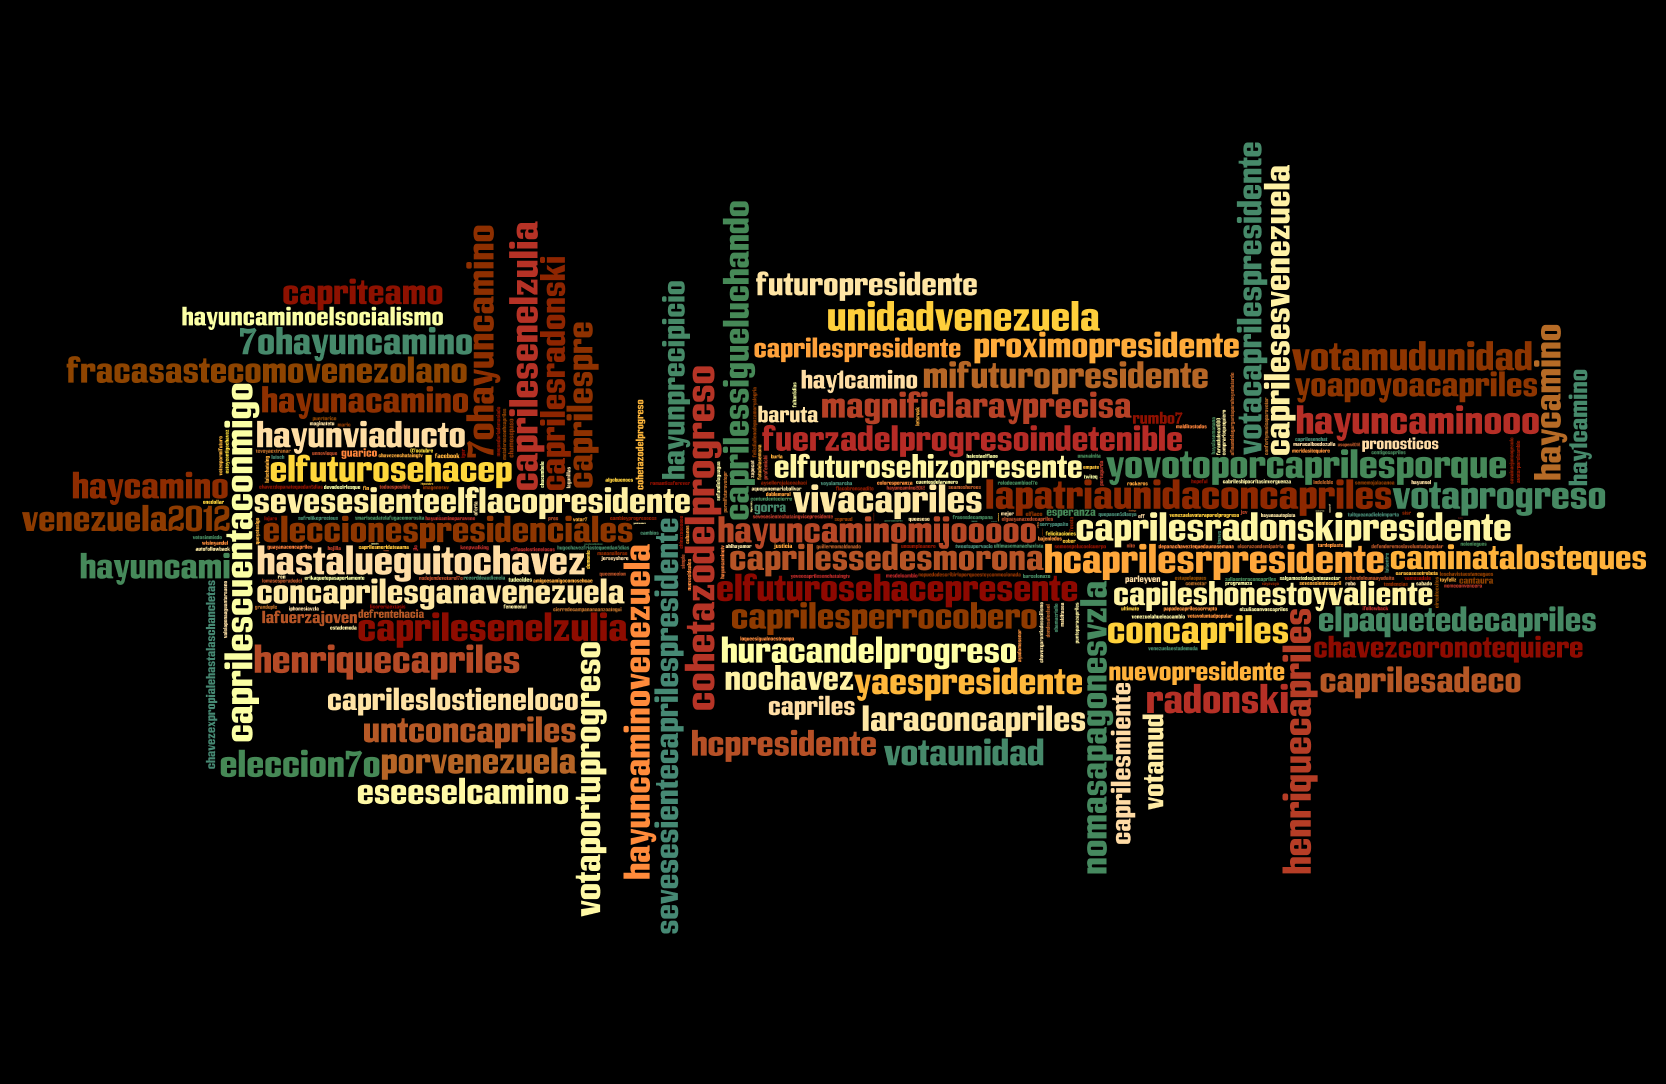
\includegraphics[width=1.0\textwidth]{support_files/caprilesWordCloud.png}
	\vspace{-1em}
	\caption{Word cloud for Henrique Capriles}
	\label{fig:caprilesWordCloud}
	\vspace{-1em}
\end{figure*}

%\newline
In this work we address this issue by building on our earlier work ~\cite{huang2012social}.
Specifically we make the following contributions:
\begin{itemize}
\item
Design and implement a new dynamic query expansion algorithm using Probabilistic Soft Logic to obtain a exhaustive vocabulary.
\item
Show how the vocabulary obtained from the Dynamic Query Expansion exercise improves the recall and accuracy of the prediction algorithms.
\end{itemize}

% word growth figure
\begin{figure*}[Ht]
	\centering
	%\captionsetup{font=scriptsize}
	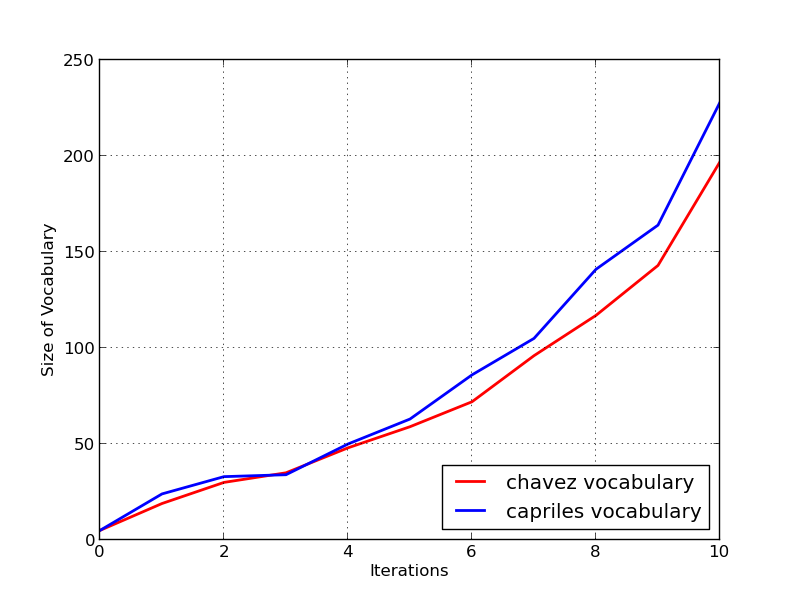
\includegraphics[width=0.7\textwidth, height=0.3\textheight]{support_files/WordGrowth.png}
	\vspace{-1em}
	\caption{Word growth over time}
	\label{fig:wordgrowth}
	\vspace{-1em}
\end{figure*}

\section{Methodology}
In most document corpora, a single concept can be referred using multiple terms.
In information retrieval (IR) this is called \emph{synonymy} and has a huge impact on the recall of documents pertaining to the concept.
Researchers address this problem by creating as exhaustive a query as possible. 
But when exploring the Twitter corpora it becomes almost impossible to hand craft such a expansive query as the meme and hashTag adaptations are not known a priori. 
\newline
To address this issue IR experts use \emph{query expansion} or reinforcement learning.
These are iterative algorithms that are initialized with a small set of query terms. 
When the documents matching the query terms are returned, after basic NLP processing such as tokenization, stop-word removal and stemming a richer vocabulary is obtained by ranking the terms in these documents by their frequency counts.
The top n words from this list is then used to query the documents again. 
The iterations are stopped when no new terms are added to the vocabulary. 
We implement such an algorithm using Probabilistic Soft Logic to build our vocabulary for a given election. 
First we review the PSL framework followed by our methodology.
% word growth figure
\begin{figure*}[Ht]
	\centering
	%\captionsetup{font=scriptsize}
	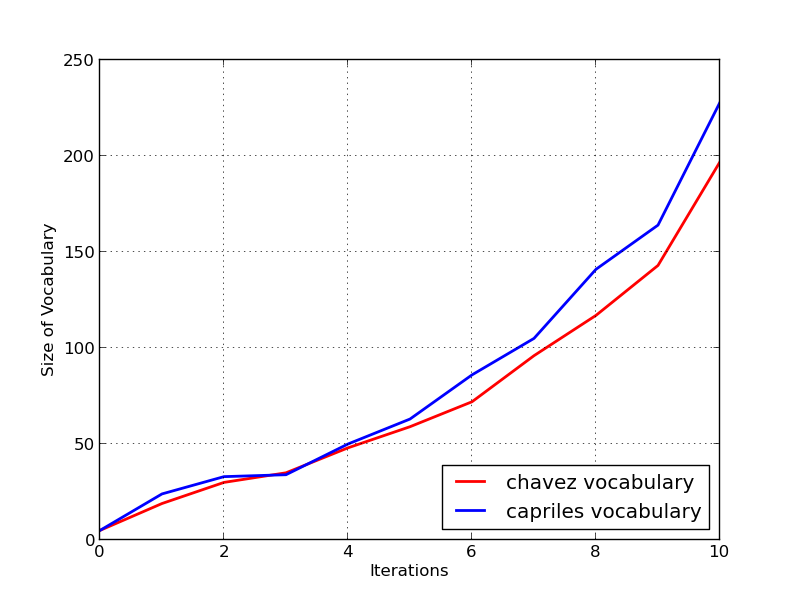
\includegraphics[width=0.7\textwidth, height=0.3\textheight]{support_files/WordGrowth.png}
	\vspace{-1em}
	\caption{Figure showing the growth of size of vocabulary for Hugo Chavez and Henrique Capriles with every iteration.}
	\label{fig:wordgrowth}
	\vspace{-1em}
\end{figure*}

\subsection{Probabilistic Soft Logic}
Probabilistic Soft Logic ~\cite{kimmig2012short} is a framework for collective probabilistic reasoning on relational domains.
PSL models have been developed in various domains, including collective classification ~\cite{broecheler2010computing}, ontology alignment ~\cite{brocheler2012probabilistic}, personalized medicine ~\cite{bach2010decision}, opinion diffusion ~\cite{bach2012scaling} , trust in social networks ~\cite{huang2012probabilistic}, and graph summarization ~\cite{memory2012graph}.
PSL represents the domain of interest as logical atoms.
It uses first order logic rules to capture the dependency structure of the domain, based on which it builds a joint probabilistic model over all atoms.
Instead of hard truth values of $0$ (false) and $1$ (true), PSL uses soft truth values relaxing the truth vlaues to the interval $[0,1]$.
The logical connectives are adapted accordingly.
This makes it easy to incorporate similarity or distance functions.
\newline
User defined \emph{predicates} are used to encode the relationships and attributes and \emph{rules} capture the  dependencies and constraints.
Each rule's antecedent is a conjunction of atoms and its consequent is a dis-junction. 
The rules can also labeled with non negative weights which are used during the inference process. 
The set of predicates and weighted rules thus make up a PSL program where known truth values of ground atoms derived from observed data and unknown truth values for the remaining atoms are learned using the PSL inference.
\newline
Given a set of atoms 
$\ell = \{\ell_1,\ldots,\ell_n\}$,
an interpretation defined as 
$I : \ell \rightarrow [0,1]^n$
is a mapping from atoms to soft truth values.
PSL defines a probability distribution over all such interpretaions such that those that satisfy more ground rules are more probable.
\emph{Lukasiewicz t-norm} and its corresponding co-norm are used for defining relaxations of the logical AND and OR respectively to determine the degree to which a ground rule is satisfied.
Given an interpretation $\mathit{I}$, PSL defines the formulas for the relaxation of the logical conjunction ($\wedge$), disjunction ($\vee$), and negation ($\neg$) as follows:

\begin{align*}
\ell_1 \softand \ell_2 &= \max\{0, I(\ell_1) + I(\ell_2) - 1\},\\
\ell_1 \softor \ell_2 &= \min\{I(\ell_1) + I(\ell_2), 1\},\\
\softneg l_1 &= 1 - I(\ell_1),
\end{align*}  

The interpretation $\mathit{I}$ determines whether the rules is satisfied, if not, the \emph{distance to satisfaction}.
A rule $\mathit{r} \equiv \mathit{r_{body}} \rightarrow \mathit{r_{head}} $  is satisfied if and only if the truth value of head is atleast that of the body. The rule's distance to satisfaction measures the degree to which this condition is violated.
 \newline
\begin{center} 
 $\mathit{d_r}(\mathit{I}) =$ max\{0,$\mathit{I(r_{body}} - \mathit{I(r_{head}}$\}
 \end{center}

PSL then induces a probability distribution over possible interpretations $\mathit{I}$ over the given set of ground atoms $\mathit{l} $ in the domain. 
If $\mathit{R}$ is the set of all ground rules that are instances of a rule from the system and uses only the atoms in  $\mathit{I}$ then,
the probability density function $\mathit{f}$ over $\mathit{I}$ is defined as
\begin{equation}
\label{eq:contimn1}
    f (I) = \frac{1}{Z} \text{exp}[-\sum_{r\in R} \lambda_r (d_r(I))^p]
\end{equation}
\begin{equation}
\label{eq:contimn2}
	Z = \int_{I} \text{exp} [ -\sum_{r\in R} \lambda_r (d_r(I))^p ]
\end{equation}
where~$\lambda_r$ is the weight of the rule~$r$, $Z$ is the continuous version of the normalization constant used in discrete Markov random fields, and ~$p \in \{1, 2\}$ provides a choice between two different loss functions, linear and quadratic.
The values of the atoms can be further restricted by providing linear equality and inequality constraints allowing one to encode functional constraints from the domain. 
PSL provides for two kinds of inferences (a)most probable explanation and (b)calculation of the marginal distributions. 
In the MPE inference given a partial interpretation with grounded atoms based on observed evidence, the PSL program infers the truth values for the unobserved atoms satisfying the most likely interpretation. 
In the second setting, given ground truth data for all atoms we can learn the weights for the rules in our PSL program.
% word cloud figure
\begin{figure*}[Ht]
\begin{center}
\subfloat[Day0]
{

\includegraphics[width=0.5\textwidth, height=0.20\textheight]{support_files/caprilesWordCloud1.png}
\label{fig:wordCloud1}
} 
\subfloat[Day6]
{
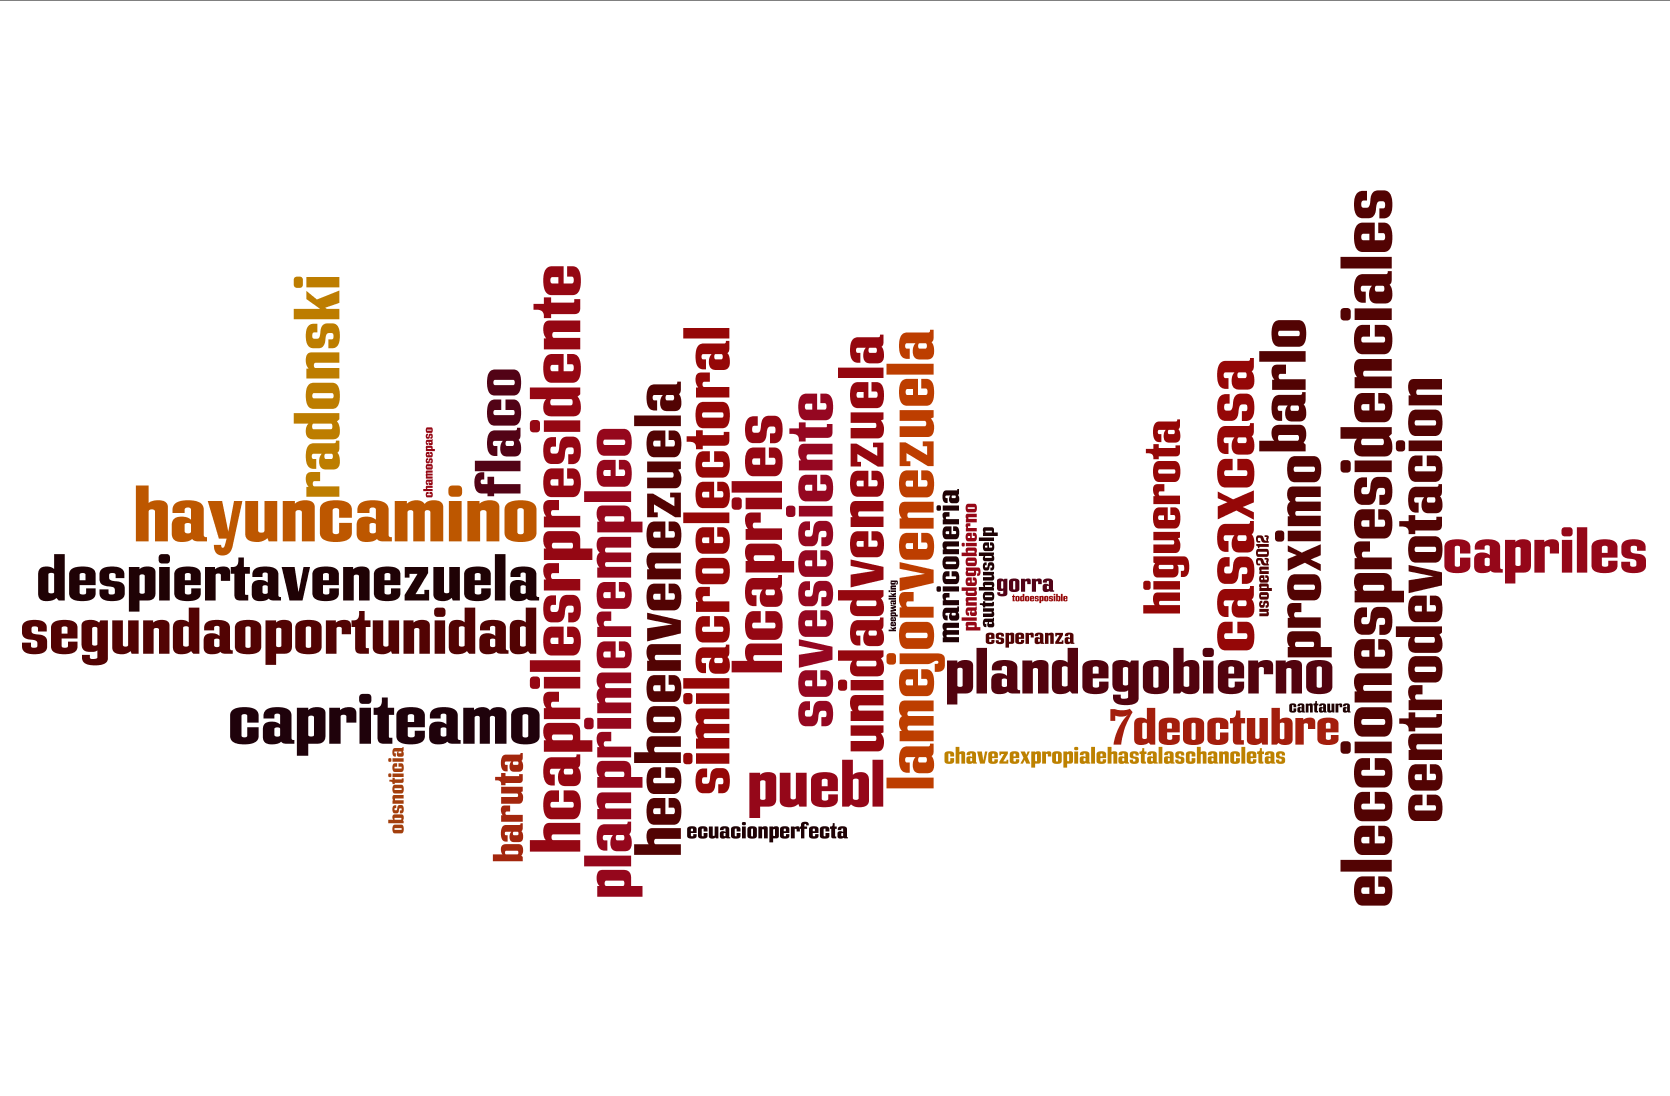
\includegraphics[width=0.5\textwidth, height=0.20\textheight]{support_files/caprilesWordCloud2.png}
\label{fig:wordCloud2}
} \\
\noindent 
\subfloat[Day15]
{
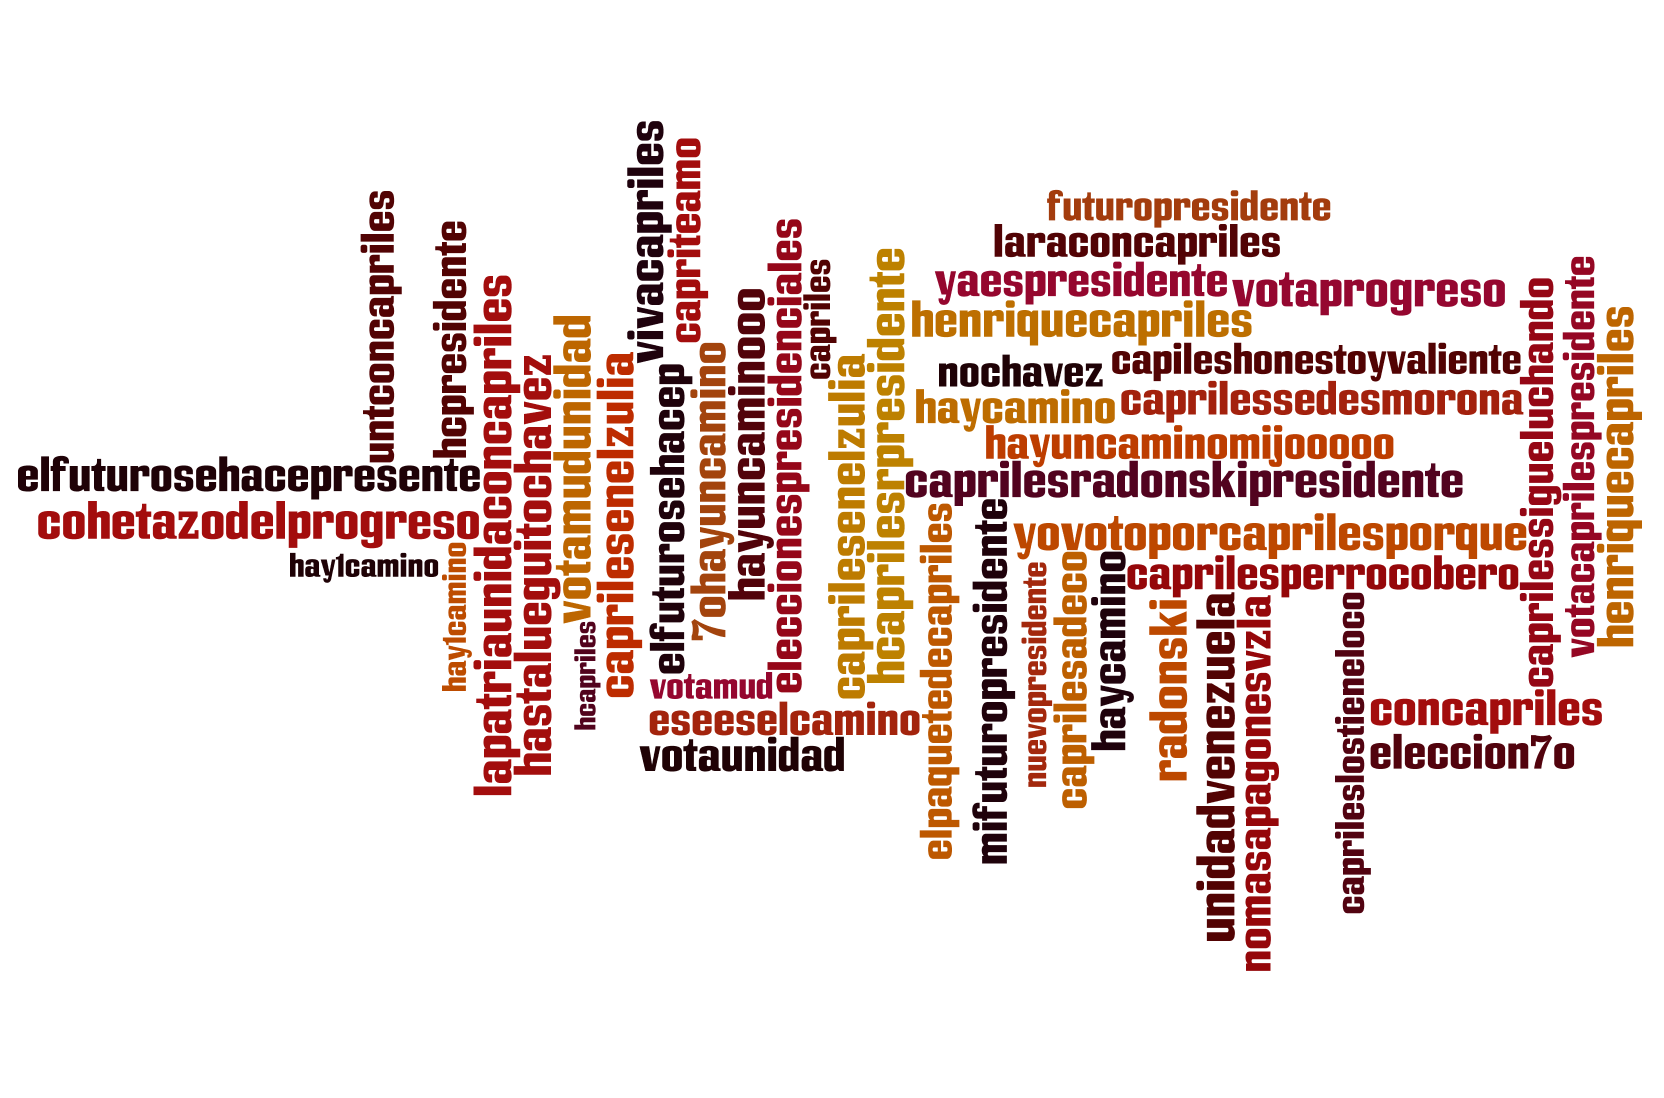
\includegraphics[width=0.5\textwidth, height=0.20\textheight]{support_files/caprilesWordCloud3.png}
\label{fig:wordCloud3}
}
\subfloat[Day30]
{
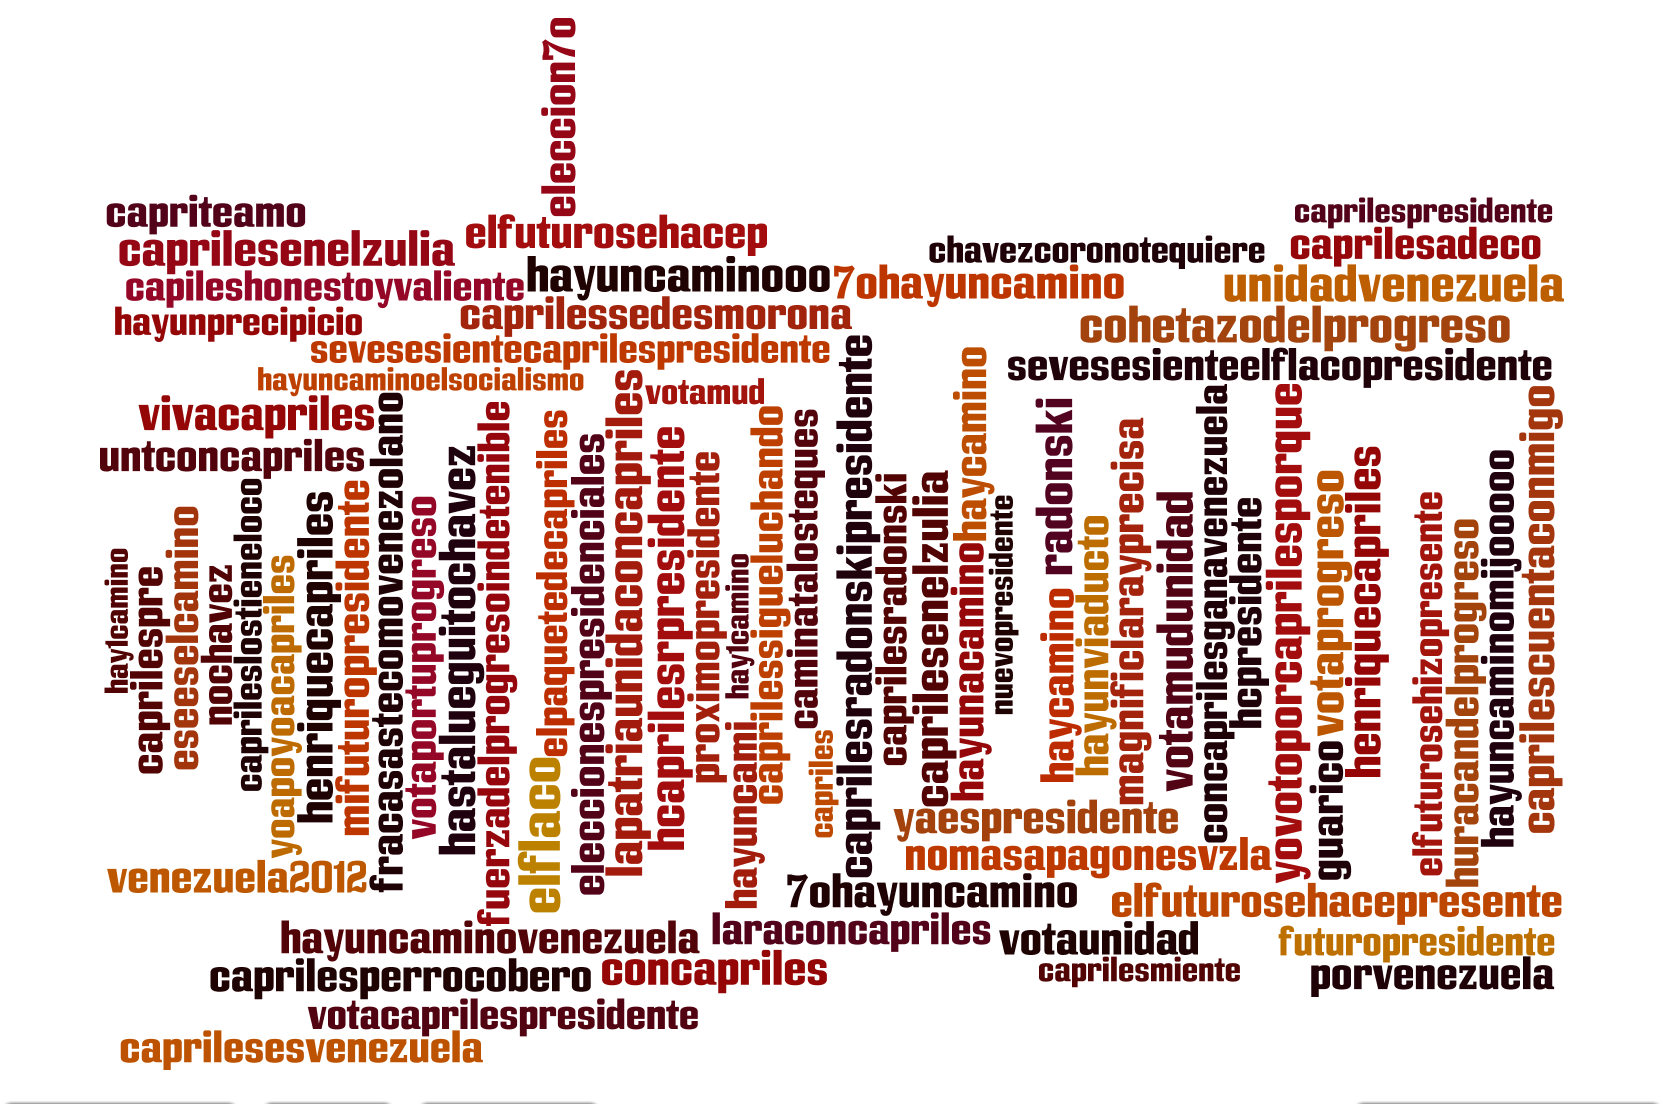
\includegraphics[width=0.5\textwidth, height=0.20\textheight]{support_files/caprilesWordCloud4.png}
\label{fig:wordCloud4}
}
\caption[caption]{Evolution of hash-tags for Henrique Capriles} 
\label{fig:wordCloud}
\end{center}
\end{figure*}
\subsection{Query Expansion using PSL}
In ~\cite{huang2012social}, we used PSL to model user affiliations within groups. 
Specifically we built a PSL program for a  social network where we have a set of users, their posts, messages to other users and the various groups we want to model. 
The rules we defined captured the dynamics of group affiliations through the various interactions.
Through the MPE inference we classified users into different groups based on their hash-tag usage and their interactions with other users.
\newline
In this paper we extend our earlier work to achieve what we call dynamic query expansion through PSL. 
Similar to the query expansion methodology described earlier we start with an initial set of key words which we believe are indicative of the affinity of a particular user to a candidate contesting in the election.
Now instead of a single inference, we iteratively perform the inference over successive time windows such that the inference from window $w_t$ is used as a prior to window $w_{t+1}$ and the inference from that is used for window $w_{t+2}$ and so on.
In order to capture the temporal connectivity between the iterations, in addition to the adaptation of rules from ~\cite{huang2012social} we define additional rules and predicates as follows:
\begin{align*}
Was\_Member(A,G) \Rightarrow Is\_Memeber(A,G)
\end{align*}
\begin{align*}
Belonged(W,G) \Rightarrow Belongs(W,G)
\end{align*}
Here the predicates $Was\_Member$ and $Belonged$ are inferences from the previous time window and are loaded in as  prior to the current iteration.
These rules are weighted slightly lower than the recursive rules below so that the system overcomes the bias it had learned in light of new more convincing evidence.
This way hash-tags that are more indicative of a user's affiliation move up in the ranking for every successive iteration and the hash-tags that aren't move down.
A similar phenomenon occurs with the user-candidate affiliations too.
Below we outline the recursive PSL rules that grows the hash-tag preferences and the user affiliations. 
\begin{align*}
\begin{split}
Tweeted(A,T) 
	\softand Contains(T,W)
	\softand Belongs(W,G) \\ 
	\softand Positive(T)
	\Rightarrow Is\_Member(A,G)
\end{split}
\end{align*}

\begin{align*}
\begin{split}
Tweeted(A,T)
	 \softand Contains(T,W)
	\softand Belongs(W,G)\\
	 \softand Negative(T)
	\Rightarrow \sim Is\_Member(A,G)
\end{split}
\end{align*}

\begin{align*}
\begin{split}
Is\_Member(A,G)
	 \softand Tweeted(A,T)
	\softand Contains(T,W)\\
	 \softand Positive(T) 
	\Rightarrow Belongs(W,G)
\end{split}
\end{align*}

\begin{align*}
\begin{split}
Is\_Member(A,G) 
	\softand Tweeted(A,T)
	\softand Contains(T,W)\\
	\softand Negative(T)
	\Rightarrow \sim Belongs(W,G)
\end{split}
\end{align*}

\begin{align*}
\begin{split}
Contains(T,W1)
 \softand Contains(T,W2)
  \softand Belonged(W1,G)\\ 
  \softand Positive(T)
	\Rightarrow Belongs(W2,G)
\end{split}
\end{align*}

\begin{align*}
\begin{split}
Contains(T,W1) 
	\softand Contains(T,W2)
	\softand Belonged(W1,G)\\ 
	\softand Negative(T)
	\Rightarrow \sim Belongs(W2,G)
\end{split}
\end{align*}

Here $Positive$ and $Negative$ are predicates whose truth values are calculated from the sentiment of the tweet such that the highly positive tweets get a truth value closer to $1.0$ for the predicate $Positive$. 
Since PSL works under the close world assumption, we do not need to specify the groundings that are false.
For tweets that do not have a positive or negative orientation we assign a truth value of $0.5$ for both the $Positive$ and $Negative$ predicates.
The last two rules are added to encode the belief that hash-tags occurring together are expected to be about the same group.
For every iteration, we collect tweets from the country of interest that was created within the time window and filter the tweets that contain any hash-tag from the previous inference  or that has been authored by or directed at a user whose affiliation is already known from the previous iterations.
\begin{table*}[Ht]
	\centering
	\begin{tabular}{| r || r | r | r | r | r | r |}
 	\hline
 	Election & UVM+Seed & UVM+PSL & Improvement & RM.+Seed & RM.+PSL & Improvement\\
 	\hline
	Mexico & 0.353 & 0.368 & -4.2\% & 0.123 & 0.07 & 43.09\% \\ 	
 	Venezuela\_Oct7 & 0.035	& 0.037 & -2.77\% & 0.158 & 0.109 & 31.01\&\\
	Ecuador & 0.531 & 0.547 & -3.01\% & 0.263 & 0.244 & 7.22\% \\
	Venezuela\_Apr15 & 0.198 & 0.178 & 10.10\% & 0.142 & 0.112 & 21.126\&\\
	Paraguay & 0.34 & 0.288 & 15.29\% & 0.2 & 0.18 & 10\% \\
	Chile\_Nov17 & 0.56 & 0.42 & 25\% & 0.245 & 0.207 & 15.51\% \\
	Honduras & 0.563 & 0.527 & 6.39\% & 0.293 & 0.184 & 37.20\% \\
	Chile\_Dec17 & 0.096 & 0.061 & 36.45\% & 0.409 & 0.369 & 9.77\% \\
 	\hline
	\end{tabular}
	\vspace{-0.5em}
	\caption{Comparison of performance of Unique Visitor Model (UVM) and Regression Model (RM) with static seed vocabulary and dynamically expanded  PSL vocabulary.}
	\label{table:improvement}
	\vspace{-0.5em}
\end{table*}	
We believe this helps us start with as little bias as possible and improve our learning with every time window.
From various experiments conducted we noticed that we get best results for a window size of 3 days. 
We begin this iterative approach by tracking tweets from 1 month prior to the election and thereby hoping to capture the changing trends in the use of hash-tags.
At the end of each iteration we are get each hash-tag's probability of belonging to a particular candidate's vocabulary. 
We normalize the each hash-tag's weight over all previous time windows so that we identify hash-tags that have remained indicative of a user's affiliation for the longest period of time without dropping in importance. 
We then use the top hash-tags ranked according to their normalized weights  for the next iteration.
This normalization reduces the influx of hash-tags that are in vogue only for a specific time window and are not as indicative of user affiliation for the entire time period. 
Figure\ref{fig:wordgrowth} shows the increase in size of the vocabulary at the end of each iteration before the normalization operation.
Figure2 shows a  the evolution  of hash-tags for Henrique Capriles.
Initially in Figure\ref{fig:wordCloud1} the system starts with only a few hand picked hash-tags that constitute the seed vocabulary. 
Then after two iterations (Figure\ref{fig:wordCloud2}) the system learns some new hash-tags like "puebl" and "higuerota". 
But these words lose importance as the learning continues because they are not very indicative of the user's preferences and  after five iterations these words drop below the threshold. 
At the same time it is also noticed that hash-tags like "capriles" and "hayuncamino" which are very strongly associated with Capriles consistently remain as the top ranked hash-tags even after ten iterations(Figure\ref{fig:wordCloud4}). 
It is also interesting to note that the algorithm identified hash-tags like "nochavez"(Figure\ref{fig:wordCloud3}) and attributed it rightly to Hugo Chavez's primary contender - Capriles. 
\TODO{Aravind}{Pick words from VE apr15 Capriles and compare to VE oct7 Capriles}
\subsection{Prediction Models}
In this section we review two prediction models we adapted from current literature to test our hypothesis. 
The first one is a naive model that forecasts elections based on the counts of mentions of a candidate.
We dub this as  \emph{"unique visitor model"} and is adapted from \cite{saez2011total} and \cite{tumasjan2010predicting}.
The second model uses a regression fit to regress from tweet features to opinion polls and then predicts election. 
This we dub as the \emph{"regression model"} and is adapted from \cite{bermingham2011using} and \cite{o2010tweets}.

\subsection{Unique Visitor Model}
Without any loss of generality, it can be assumed that large parties that are more popular will have a larger social media foot print than smaller and less popular parties. 
This model takes advantage of this assumption and predicts elections by calculating the relative popularity of candidates contesting the election.
We first define a vocabulary for each candidate. 
This vocabulary is crafted by hand and includes the candidate's names and aliases, the name and acronyms for his/her political party and the official Twitter handle of the candidate.
For the given time period, the tweets from the country in question are tracked for the occurrence of the terms in the vocabulary.
We then build a time series of sentiment and klout scores from the tweets returned.
Klout score is a value provided by Klout.com that quantifies the impact each user has on social media. 
We use the sentiment scores provided as a part of the meta-data of the tweet. 
%The sentiment scores typically fall in the range of $[-15,15]$ and is provided by Lexalytics - a pioneer in linguistic processing.
Once a time series of the klout and sentiment time series are built, we calculate the absolute popularity of a candidate by summing the product of the klout score of the user and the average sentiment value of tweets from the user mentioning the candidate.
% $C_d$ as:
%\begin{equation}
%{C_d} = \sum_i K_i * UCS_{id}
%\end{equation}
%where $K_i$ is the klout score for user $i$, and $UCS_{id}$ is User Candidate Score, the average of sentiment scores for all tweets from user $i$ about candidate $d$.
We then normalize the popularity scores across all candidates so that they sum to $1$.
This gives us the relative popularity of each candidate %$P_d$
using which we predict the elections.
%\begin{equation}
%{P_d} = \sum_i \frac{C_d}{C_i}
%\end{equation}
%From the above equations, 
We calculate the absolute popularity such that each user contributes only once to the popularity score of a candidate.
This was preferred to merely counting the mentions of a candidate so as to remove the bias of bot generated tweets from election campaigns that boosted the number of times a candidate is mentioned on Twitter.
\subsection{Regression Model}
\aravind{should i completely remove the equations from regression model too? its easier to explain with them}
In this model, in addition to Twitter data, we leverage the opinion polls available for the elections to make our predictions.
Like the earlier model we track the tweets that contain a word from the vocabulary defined for each candidate.
We then define a linear regression fit that uses the opinion polls as dependent variable and features generated from these tweets as independent variable.
We use a total of 6 features based on klout scores, number of unique users, total number of mentions, sentiment and incumbency.
We normalize each of these features across all candidates to get the relative share of the volume. 
For example for the we define share of positive mentions($SoPM$)  as: 
\begin{equation}
SoPM(x) = \frac{\#PositiveMentions(x)}{\sum_i \#PositiveMentions(i)} 
\end{equation}
and share of negative users($SoNU$) as:
\begin{equation}
SoNU(x) = \frac{\sum_j K_j}{\sum_i \sum_j K_j}
\end{equation}
where $K_j$ is the klout score of user $j$ who tweeted about a candidate.
Similarly we define share of sentiment ($SoS$) as the sum of all sentiment scores normalized across all candidates. 
We use a binary variable for incumbency. 
We then build a time-line of opinion polls. 
For each of the polling dates we calculate these features by using tweets created during the 10 day window leading up to the polling date.
When we have more than one polling house publishing its opinion poll for the same date we take the average of the polls. 
Once we create a feature set for all the polling dates, we fit a simple least square regression as :
\begin{equation}
\begin{split}
Popularity(x) = \alpha_1 * SoPM(x) + \alpha_2 * SoNM(x) \\
						 + \beta_1 * SoPU(x) + \beta_2 * SoNU(x) \\
						 + \gamma * SoS(x) + \delta * Incumbency(x) + \epsilon
\end{split}
\end{equation}
From the  weights learned from the regression fit we confirm that the sentiment and number of unique users have more predictive power than the number of mentions.	
After learning the regression fit, we make a prediction by building such features using tweets from the 10 day window leading up to the prediction date.
\begin{figure*}[Ht]
	\centering
	%\captionsetup{font=scriptsize}
	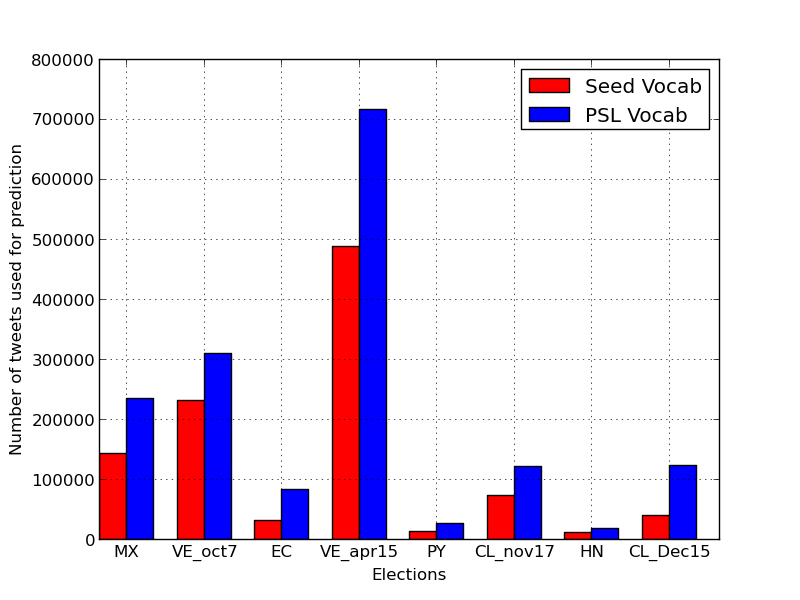
\includegraphics[width=0.7\textwidth, height=0.3\textheight]{support_files/Recall.png}
\vspace{-1em}
	\caption{Recall of seed vocabulary vs PSL vocabulary}
	\label{fig:recall}
	\vspace{-1em}
\end{figure*}

\section{Results}
To evaluate our hypothesis we test our models on different elections from Latin America.
The tweets are provided by DataSift, an infoveilence service that resells Twitter data.
On an average we collect close to 2 million unique tweets a day from over 21 countries in Latin and South America.
Then these tweets are geo-coded using a geo-location algorithm we developed to obtain tweets from the country of interest.
We then run the two prediction algorithms to get their baseline performance.
These two models have been tested extensively on 36 elections from Latin America from 2012-2013 including Presidential, Governor and Mayoral elections. 
Out of these 36 elections, the models predicted 21 of them correctly. 
%The combined track record for the two elections have been detailed in \ref{table:trackRecord}. 
Importantly every single election was predicted ahead of time and not in retrospect.
The models perform poorly on local mayoral elections(12 out of 24 predicted correctly) as there was not much chatter on Twitter about these elections to make sound predictions. 
The regression model was used only for presidential elections as opinion polls were not available for Governor and Mayoral elections.
Hence we use only the presidential elections to evaluate our vocabulary.
Once we have the baseline score for these models, we then use the same vocabulary to seed our PSL learning algorithm. 
The prediction algorithms are then run again, now by using the expanded vocabulary obtained through the query expansion at each iteration.

Figure \ref{fig:recall} shows the increase in the number of documents that were used by the algorithm to make a prediction.
It is noticed when averaged across all the 8 elections we have close to a 2x increase in the number of tweets that were used by these models.
This is a substantial increase in the recall of relevant tweets for the domain.
To further illustrate the fact that the vocabulary used by such algorithms plays a vital role, we compare the performance of the models using the two different vocabularies.
The Mean Absolute Percentage Error (MAPE) was used as a metric to measure the performance of the models. 
To reduce the effect of outliers we track the popularity of only the major candidates and ignore the ones who obtained less than 10\% of the total votes.
Table \ref{table:improvement} shows the performance of each vocabulary in different elections. 
On an average it is seen that the mean absolute percentage error is reduced by 16.13\%.
We see greater improvement with the regression model as the model weights each window of tweets differently depending upon the opinion poll time series whereas the unique visitor model values them equally. 
Therefore, when the algorithm picks up 'not-so-informative' hash-tags during the earlier iterations, the sentiment value and the counts of these mentions bring down the accuracy of the model even though at a later stage hash-tags that are strongly indicative of a user's preference is picked up. 

\section{Conclusions and Future Work}
In this work we built a novel query expansion methodology using Probabilistic Soft Logic.
We showed how such a vocabulary has a direct impact on the recall of documents and the accuracy of prediction algorithms.
%Specifically we were on an average able to reduce the MAPE error of election prediction algorithms by 15.58\%.
It is important to note that though we used elections to show performance gains, the query expansion system is generic and can be used to learn a vocabulary for any given domain.
Further, this work is motivated towards a future goal to model the electorate demographics.
With more fine grained data about the gender, age and exact location of a user it is possible to infer the preferences at a group level rather than at a user level.
This would enable us to study the various interactions between groups and individual users in more detail and thus make more informed election predictions.
\linebreak
\textbf{Acknowledgments}
This work is supported in part by the National Science Foundation under Grant No. 0937094 and the Intelligence Advanced Research Projects Activity (IARPA) via Department of Interior National Business Center (DoI/NBC) contract number D12PC00337. The U.S. Government is authorized to reproduce and distribute reprints for Governmental purposes notwithstanding any copyright annotation thereon. Disclaimer: The views and conclusions contained herein are those of the authors and should not be interpreted as necessarily representing the official policies or endorse- ments, either expressed or implied, of IARPA, DOI/NBA, or the U.S. Government.
\linebreak
\linebreak
\linebreak
\linebreak
%\pagebreak
\bibliographystyle{AuthorKit/aaai}
\bibliography{references}
\end{document}
